\documentclass[11pt]{article}
\renewcommand{\baselinestretch}{1}

% PACKAGES
%-----------------------
\usepackage[left=3cm, right=3cm, top=3cm, bottom=3cm,nohead,nofoot]{geometry}
\usepackage[T1]{fontenc}
\usepackage[utf8]{inputenc}
\usepackage{amsmath}
\usepackage{listings}
\usepackage{graphicx}
\usepackage{pdfpages}
\graphicspath{{plots/}}
\usepackage{float}
\usepackage{wrapfig}
\usepackage{caption}
\usepackage{url}
\usepackage{hyperref}
\usepackage{graphics}
\usepackage{caption}
\usepackage{subfigure}
\usepackage[parfill]{parskip}



% DOC INFO
%-----------------------
\title{MirrorTrees: Protein-	interactins through the looking-glass}
\author{
	Sergio Castillo
	\and
	Joan Martí
	\and
	Adrià Pérez
}
\date{Structural Bioinformatics, MSc in Bioinformatics for Health Sciences - Universitat Pompeu Fabra}

% DOCUMENT
%-----------------------
\begin{document}
\maketitle

\section{Introduction}
In the so-called OMICS era, with the high-throughput techniques, the amount of data is huge. This is not an exception of proteomics data. Nowadays, huge databases for proteins exist, at distinct levels (inferred, detected, crystallised, etc). However, there is still a gap concerning the interaction between proteins. This lack of knowledge is due to the fact that proteic physic interactions used to be found by experimental means (immunoprecipitations, double-hybrid, etc).


Now, there is an opportunity to infer physical interactions \textit{in silico}, and then focus the experimental work to validation.

There are different algorithms or procedures for inferring proteic physical interactions, but in this essay we are going to cover only the MirrorTree approach, developed in early century by Dr. Alfonso Valencia and associates \cite{Pazos2001}.


The MirrorTree approach is based on co-evolutionary methodology, as this technique assumes that if two proteins interact physically, they should co-evolve and they should share similar evolutionary history.



\section{Methods}
\subsection{MirrorTree}
The MirrorTree methodology, developed by Dr. Alfonso Valencia and associates, predicts direct interactions between proteins based on co-evolution of interacting proteins. \cite{Pazos2001}. The work-flow of this method is as follows:
\begin{enumerate}
\setlength{\itemsep}{1pt}
	\item Gather \textit{n} sequences to test their interactions.
	\item Look for the orthologous sequences for each protein query (search by homology, using BLAST \cite{BLAST}).
	\item Build an MSA for each protein query.
	\item Build distance matrix for each set (using McLachlan71).
	\item Compare the the distance matrices at 1:1 rate.
	\item Compute the correlation coefficient (Pearson's r) based on the difference between the matrices.
	\item Infer interaction.
\end{enumerate}
MirrorTree is settled upon the following suppositions:
\begin{enumerate}
\setlength{\itemsep}{1pt}
	\item Proteins that interact directly co-evolve.
	\item Proteins that interact directly and co-evolve should share the same evolutionary history, so they must have similar phylogenies.
\end{enumerate}
In further sections there would be a discussion over these assumptions.

\subsection{mtree}

Our integrative tool takes a slightly different approach to the Valencia's team to MirrorTrees. \texttt{mtree} takes a list of animal sequences in FASTA format and predicts protein-protein interactions between them.

First, \texttt{mtree} performs a \texttt{jackhmmer} to search for homologous proteins for each query sequence. The program uses three iterations and then saves the resulting hidden markov models generated by \texttt{jackhmmer}. Only one homologous sequence is selected for each species, to avoid building phylogenetic trees using paralogous. The sequence with the lowest e-value for each species is used by the program.

After doing this, \texttt{mtree} considers all the possible pairs of sequences that have homologs in at least \texttt{k} common species, where \texttt{k} can be changed using the option \texttt{-sp}. The program uses a default value of \emph{10} for \texttt{k}, as similar values were used by Pazos and Valencia \cite{Pazos2001}.


In order to predict interactions, \texttt{mtree} performs an MSA for each query sequence and its homologs using \texttt{hmmalign} and the hidden markov models generated by \texttt{jackhmmer}. Then, a distance matrix is built using the BioPython module \texttt{Phylo::TreeConstructor}. Pearson's correlation coefficient and Spearman's rho is computed for each pair of matrices. 

\texttt{mtree} uses an alignment of 18S rRNA downloaded from the SILVA database \cite{SILVA} and also computes a distance matrix for each interaction candidate. Then, the program performs a partial correlation of the matrices of the two query sequences, controlling for the rRNA distance matrix. This procedure, derived from the methodology used by Sato et al. \cite{Sato2005}, has the goal to isolate the coevolution effect from other spurious correlations; namely, the intrinsic correlation between two distance matrices due to the evolutionary history of the species involved.

In the end, \texttt{mtree} reports three measures for each interacting pair candidate:

\begin{enumerate}
\setlength{\itemsep}{1pt}
	\item \textit{Pearson's r}\cite{Pazos2001}.
	\item \textit{Spearman's rho:} As maybe the relationship between matrices is not linear, or it may have 		outliers that alter the fitting of the linear model, it could be of help to see how a rank-based correlation performs.
	\item \textit{Partial correlation (using 18S rRNA phylogeny of the species):} When 			computing the correlation between the matrices, there exists a common relationship that needs to be taken into account: 		the phylogeny of the species used in the trees. For building the phylogeny a lineage-specific marker is 		needed. Usually it is recommended to use the 18S rRNA for these purpose\cite{Sato2005}.
\end{enumerate}

The user can provide a Pearson's correlation cutoff to label the predictions, and \texttt{mtree} will print the results in tabular format. Also, a representation of the predicted interaction graph can be created using Cytoscape.js \cite{Franz15012016}  if given the option \texttt{-g}.



\subsection{Evaluation}

In order to develop mtree, different train/test sets were built. For doing so, it is important to know beforehand the relationship between proteins, that is, if each pair of sequences really interact or not.

The IntAct database\cite{intact} is a curated database for known interactions between proteins. Downloading the dataset (2012-10-16 release) in MITAB27 format (extension from PSI-MI format).

The Negatome database\cite{negatome} is a curated database for proteins that do not interact under experimental conditions. It has its own tabular format. For ensuring its reliability, the most stringent dataset was downloaded (\textit{manual-stringent.txt} 2014 release), which is manually curated and filtered against IntAct information.

The sequences where retrieved by Uniprot ID from the local Uniprot database (previously downloaded in FASTA format and filtered). 

Both datasets are useful for assessing known interactions (IntAct) and known non-interactions (Negatome), and therefore, checking the reliability of \texttt{mtree} predictions.

Multiple sequence alignments of 18S rRNA of species used in previous steps were needed. We downloaded the alignment from the SILVA database\cite{SILVA} (release 123), using the full alignment (but truncated by the aligned region).

Interacting and non-interacting sequences were filtered by the species contained in the alignment from SILVA, as well as the local Uniprot database, for increasing the performance of \texttt{mtree}.



\section{Discussion}
Despite being a possible theoretical approach, Valencia's work in 2001\cite{Pazos2001} needs to be improved and analysed. The approach here presented has prominent differences with the reference work. In the following sections there are specified which points needed to be changed and the reasons for doing so.

\subsection{Assumptions}
One of the main handicaps that exist in the MirrorTree method is that its assumptions are not always valid.
\begin{enumerate}
\setlength{\itemsep}{1pt}
	\item \textit{Proteins that interact directly co-evolve}: Not necessarily. Interaction between proteins 		occurs at domain level, more precisely it interacts with the interaction region, a smaller region within 		the domain, not at the whole protein. It might be true that interaction regions co-evolve, but that does 		not mean that co-evolve the whole protein. Besides, even the co-evolution between interaction sites is 		somehow obscure, as it depends on the intensity of the selective pressure between them. It is known that 		the interaction between proteins is not static, is partially adaptative (key-lock vs greeting-hands). So, 	would always be relevant an aminoacid exchange? How intense is the selective pressure between the 			regions?

	Moreover, co-evolution can also act at network level, therefore, it is plausible that proteins that do 		not physically interact may co-evolve, as both might be of importance in the pathway. Then, does proteins 	can de detected as false positive, as they interact, they have a relationship but not interact directly. 		Co-evolution is a good measure for direct interaction?

	\item \textit{Proteins that interact directly and co-evolve should share the same evolutionary history, 		so they may have similar phylogenies.} This is a strong assumption, as it would be commented in following		sections, co-evolution relies upon strong selective pressure in order to be fully detected. In order to 		have coincident phylogenies, there should be a fairly strong selection between interactors. The problem 		raises as this is not a frequent.
\end{enumerate}

\subsection{Search of orthologs}
One of the main difficulties when working with phylogenies, and by extension to this essay, is the difficulty to distinguish orthologs from paralogs, one of the paradigmatic problems on the field. 

When retrieving orthologous sequences, paralogous sequences are also retrieved. As they refer to different events of diversification (species vs. gene respectively), there is an introgression of another relationship within our model, adding confounding relationships, and therefore decreasing the predictive power of the approach.

Besides, proteins, and in special, proteins from multicellular eukaryots, may have many domains. If the aim of the study is to asses direct interaction between proteins, it must focus on the interaction region. Using BLAST-based searches can also lead to misleading homology, as it might search homologous sequences based on a domain which is not related to the interaction.

On the contrary, HMM-based searches look for homologous sequences using hidden markov models, which may improve the search for holomogs. For this reason, mtree uses HMM-based searches instead of BLAST-based searches.

\subsection{Weight Matrix}
The distance matrix can be computed using different weight matrices (e.g. Blosum62, McLachlan71, Dayhoff Pam Matrix, etc.) or distance correctors (p.e. Kimura's distance). Despite being a variable in the approach, some authors\cite{Zhou13} have found that its change does not provide an improvement of the prediction power.

This might be true due to that the focus of MirrorTree is to compare between trees (a.k.a distance matrix). The relevant point is to use the same statistic in both MSAs, not in how good or accurate is the estimation of the distances.

In order to see which of them provided a better classification for interactions between proteins, all three statistics are taken into account by mtree.

\subsection{Reproducibility}
One of the reported problems about the MirrorTree approach is the reproducibility. Above all, the goodness of the results depend on the chosen dataset. As observed in Zhou's work\cite{Zhou13}, 3 different sets, with reasonable resemblance between them:
\begin{enumerate}
\setlength{\itemsep}{1pt}
	\item \textit{Set1:} Common interactors of \textit{Saccharomyces cerevisiae} and \textit{Homo sapiens}, 		with both cases experimentally confirmed their interaction.
	\item \textit{Set2}: Analogous but pairs only need to be experimentally confirmed in one of the two 			species.
	\item \textit{Set3}: Analogous to set1 but using common interactors of \textit{Mus musculus} and   \textit{Homo sapiens}).
\end{enumerate}
Only certain degree of differences between interacting pairs and non-interacting pairs can be seen in set1. Set2, a more stringent subset of set1, does not show any difference between both groups, and set3, which is analogous to set1 but using more evolutionary closed species, neither shows it.

In addition, in Valencia's article\cite{Pazos2001} 3 datasets are used:
\begin{enumerate}
\setlength{\itemsep}{1pt}
	\item \textit{Set1:} Interacting Domains.
	\item \textit{Set2:} Interacting Proteins of bacteria.
	\item \textit{Set2:} Interacting Proteins by genome.
\end{enumerate}

The results of the set1 (domains) is highly controversial, as it predicts better the co-evolution between domains of the same protein (logic if within protein selective pressure is taken into account) than between interacting domains. As previously mentioned, maybe the selective pressure, and thus the co-evolution is laxer in interacting domains than in within protein domains. Therefore, is co-evolution a good measure of selective pressure in protein interaction?
In set2, it seems to be possible to properly classify the interactions (despite counting with ambiguous classification \textit{possible}). In set 3 the situation is analogous to set2.


\section{Results}
\subsection{Mutual information}
In order to know which coefficient is better for the predictions, mutual information (MI) was computed using the R package \textit{FSelector} (version 0.19). MI is used when comparing the relative importance of different features with respect a classification variable. In our case, the classification variable has two classes (interacting or non-interacting), and we had three features (Pearson's coefficient, Spearman's rho and the partial correlation coefficient). 

The mtree result confirmed the expectations, non of the coefficients was a strong predictor for the interactions in our evaluation dataset.

\subsection{Data}

% ESTO DEBERIA ESTAR EXPLICADO EN EVALUATION. Ademas no se entiende muy bien lo de los animales.
%The set of available animals was restricted to the \textit{animals} taxon, 200 sequences that interact and 80 sequences that do not interact. The results for our three measures (Pearson's r, Spearman's rho and partial correlation coefficient) are represented in Fig. 1, separating real interactions from IntAct (YES) and false interactions from Negatome (NO).

As it can be seen in Fig.1, the predicting power of \texttt{mtree} using Pearson's correlation coefficient is better than chance, with a precision of 0.78 and a recall of 0.12. However, our dataset was not balanced, and the precision fell to around 0.6 when correcting for the differences in number between true interactions and false interactions.

Despite the fact that some authors\cite{Sato2005} reflect that correcting the correlation by partialing out the phylogenetic relationship enhances the MirrorTree approach, with our dataset that is not the case, as the partial correlation coefficient is very high for both groups of interactions.

Therefore, despite using different coefficients, \texttt{mtree} is only able to make weak predictions. As it is commented in the following section, there is an important lack of reproducibility of Valencia's approach \cite{Pazos2001}, not only by \texttt{mtree} but also by other authors. 



\section{Conclusions}
Aqui un resumen/conclusiones/final remarks.

\begin{figure*}[t]
	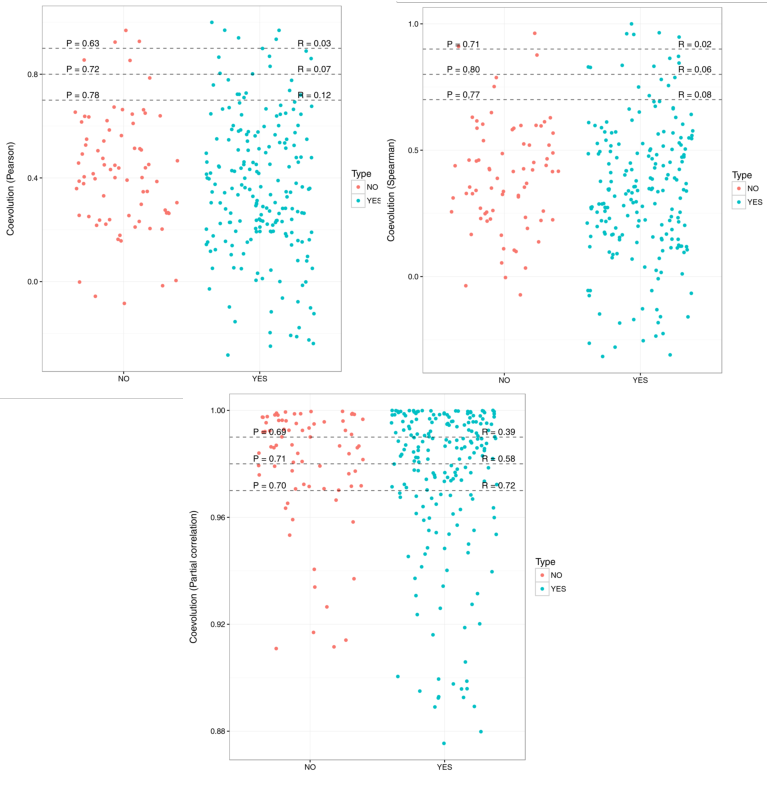
\includegraphics[width=1.0\textwidth]{graphics3}
	\enspace \caption{Relationship between the correlation coefficients and the labelling success. In each plot we can find the distribution of each of our measures on true interactions from IntAct (YES) and non-interacting proteins from Negatome (NO). The dotted lines represent different cut-offs for labelling the interactions as true, and above each line we can find the precision (P) and the recall (R) for that particular classification.}
\end{figure*}

\bibliographystyle{ieeetr}
\bibliography{project}	
\end{document}
